\section{Cifrari storici}
Sono nati per comunicazioni "sicure" ristrette a poche persone. Cifratura e decifratura eseguite con carta e penna ed un alfabeto di 21 o 26 lettere. Tutti i cifrari storici rispettano i principi di \emph{Ruggero Bacone} che dicono:
\begin{itemize}
    \item cifratura e decifratura devono essere eseguibili facilmente
    \item deve essere impossibile decifrare il messaggio senza conoscere l'algoritmo
    \item il crittogramma deve apparire innocente
\end{itemize}

\subsection{Cifrario di Cesare}
Il cifrario di Cesare è il primo di concezione moderna, tuttavia è senza chiave. La sua sicurezza si basa sulla ristrettezza di chi lo conosce. Si può generalizzare scegliendo un $k$ arbitrario che indica di quanti posti dobbiamo ruotare l'alfabeto, in questo caso $k$ sarebbe la chiave. 

Indichiamo con $pos(x)$ la posizione di $x$ nell'alfabeto, per cifrare si deve quindi sostituire $x$ con:
$$ y : pos(y) = pos(x) + k \mod 26 $$
per decifrare si sostituisce $y$ con:
$$ x : pos(x) = pos(y) - k \mod 26 $$

NB: si suppone che $pos('A') = 0$

NB: fisicamente questa sostituzione si otteneva tramite disci concentrici in cui:
\begin{itemize}
    \item il disco interno contiene le lettere dell'alfabeto in chiaro
    \item il disco esterno contiene le lettere cifrate
\end{itemize}

Si può forzare facilmente in quanto le chiavi sono poche e si può brutare. Questo cifrario gode della proprietà commutativa cioè: data una sequenza di chiavi e di cifrature cambiando l'ordine in cui le eseguiamo non si varia il crittograma finale. In fine vale:
$$ C(C(s, k_2), k_1) = C(s, k_1 + k_2) $$

Comporre più cifrature quindi non aumenta la sicurezza del sistema!

Questo cifrario appartiene alla classe dei \emph{cifrari a sostituzione} cioè quelli in cui ogni lettera viene scambiata con un'altra o più di una seguendo un determinato ordine.

\subsection{Cifrari a sostituzione}
Si dividono in:
\begin{itemize}
    \item \emph{monoalfabetici}: un carattere si sostituisce sempre con lo stesso carattere
    \item \emph{polialfabetici}: un carattere si sostituisce con più di un carattere in base al contesto nel quale appare
\end{itemize}

\subsubsection{Cifrario affine}
$$ x \xrightarrow{} y : pos\left(y\right) = a \cdot pos\left(x\right) + b \mod 26 $$
$$ K = <a, b> $$

Per far funzionare la decriptazione $a$ e $b$ vanno scelti in maniera particolare:
\begin{itemize}
    \item $a$ va scelto invertibile cioè deve esistere $a^{-1} : a \cdot a^{-1} \mod 26 = 1$, questo si ottiene \emph{se e solo se} $MCD(a, 26) = 1$. Più in generale $a \in \mathbb{Z}$ è invertibile in $\mod m$ \emph{se e solo se} $MCD(a, m)=1$
    \item $b$ si può scegliere a piacere
\end{itemize}

La decriptazione si effettua quindi con:
$$ y \xrightarrow{} x : pos\left(x\right) = a^{-1} \cdot (pos\left(y\right) - b) \mod 26 $$

con $a \cdot a^{-1} \mod 26 = 1$

NB: scegliendo $a$ primo si vince sempre

Es: $K = <13, 0>$: tutte le lettere in posizione pari verrebbero trasformate in 0 e tutte quelle di posizione dispari diventano 13. E' quindi importante scegliere a: $MCD(a, 26)=1$

Proviamo a contare le possibili chiavi tale che $a$ e 26 sono coprimi:
$$ 26 = 2 \cdot 13 $$
$$ a \in \{ \text{dispari tra 1 e 25 tranne 13} \} \xrightarrow{} 12 \text{ valori possibili} $$
$$ \text{b scelto a piacere tra 0 e 25} \xrightarrow{} 13 \text{ valori possibili } $$
abbiamo quindi in totale 312 chiavi (311 perché $<1,0>$ lascia inalterato il testo).

Se la segretezza dipende unicamente dalla chiave allora il numero delle chiavi deve essere così grande da essere immune da tentativi di ricerca esaustiva e poi va scelto in maniera casuale.

\subsubsection{Cifrario completo}
Generiamo una permutazione a caso dell'alfabeto e la usiamo come chiave.
$$ \text{lettera in chiaro di posizione i} \xrightarrow{} \text{lettera di posizione i nella permutazione} $$

Quante possibili chiavi ci sono? Una chiave è una permutazione di 26 lettere, lo spazio delle chiavi è per tanto $26! - 1 \text{ } (~4 \cdot 10^{26})$

Questo grande spazio di chiavi tuttavia non è sufficiente a dire che il sistema è sicuro in quanto rimane vulnerabile sfruttando:
\begin{itemize}
    \item strutture logiche dei messaggi in chiaro
    \item occorrenza statistica delle lettere
\end{itemize}

\subsection{Cifrari a sostituzione polialfabetica}
Una stessa lettera incontrata in punti diversi del messaggio in chiaro ammette un insieme di lettere sostitutive possibili scelte con una determinata regola.

\subsubsection{Archivio fotografico di Augusto}
Non veniva usato per comunicare ma per mantenere un archivio di informazioni cifrato. Ritrovata dopo la sua morte fu svelata dall'imperatore Claudio:
\begin{itemize}
    \item i documenti erano scritti in numero, non in lettere
    \item Augusto scriveva i messaggi in greco, poi metteva in corrispondenza la sequenza di lettere del documento con la sequenza di lettere del primo libro dell'Iliade
    \item sostituiva ogni lettera del documento con il numero che indicava la distanza tra le due lettere di pari posizione
\end{itemize}

Il cifrario è stato forzato perché Claudio ha trovato il libro di Augusto ed ha notato scritture, calcoli ed annotazioni.
Questo è un cifrario molto sicuro se la chiave è lunga o si cambia sempre libro in uso o porzione del libro.

\subsubsection{Disco di Leon Battista Alberti (XV secolo)}
Abbiamo due disci ruotanti:
\begin{itemize}
    \item quello esterno ha delle lettere (non tutte) e numeri, e si usa per formulare il messaggio
    \item quello interno, più ricco, ha la disposizione delle lettere in maniera arbitraria e diversa per ogni coppia di utenti
\end{itemize}

\begin{verbatim}
    ABCDEFGHILMNOPQRSTUVZ12345
    SDTKBJOHRZCUNYEPXVFWAGQILM
    Chiave: A-S
    messaggio: NON FIDARTI DI EVE
    m = NONFIDA 2 RTIDIEVE
    c = UNUJRKS Q UYBMBSPS
    quando si arriva su 2 la chiave diventa A-Q
\end{verbatim}

Quando si decifra si decifra partendo con la chiave A-S, arrivando alla Q si nota che si ottiene 2, quindi va cambiata la chiave.

C'è un secondo modo per usare questi dischi: il metodo dell' \emph{indice mobile}:
\begin{verbatim}
    ABCDEFGHILMNOPQRSTUVZ12345
    EQHCWLMVPDNXAOGYIBZRJTSKUF
    m: ILD 2 EL P FINO
    c: PDC S WD O OIRJ
\end{verbatim}

Inizialmente la chiave è A-E, poi decifrando si trova 2: tra due letteresi cambia chiave. Si decifrano quindi altre 2 lettere nella giusta maniera e la lettera dopo sarà P cioè la nuova chiave A-P e successivamente si inizia a decifrare con questa nuova chiave.

In genere si cambia chiave ogni volta che si trova un carattere speciale. Inserendoli spesso il cifrario è difficle da attaccare se la chiave viene cambiata ad intervalli imprevedibili.

NB: La macchina Enigma è una versione elettromeccanica del cifrario di Alberti.

\subsubsection{De Vigenère}
E' una estensione della tecnica dell'Alberti più sicura che è rimasta irrompibile per 3 secoli. Si sceglie una chiave in cui ogni lettera corrisponde ad un numero che sarà di quanto bisogna shiftare il testo in chiaro per ottenere il testo cifrato:
\begin{table}[ht!]
    \centering
    \begin{tabular}{c c c c c c}
        C & H & I & A & V & E \\
        2 & 7 & 8 & 0 & 24 & 4
    \end{tabular}
\end{table}
la chiave si ripete tante volte quanto serve per equiparare il messaggio in lunghezza:
$$ NONFIDARTIDIEVE $$
$$ CHIAVECHIAVECHI $$
$$ PVVFGHCYBIBMGCM $$

Si può vedere anche con una matrice 26x26 in cui ad ogni incrocio si trova la lettera $i$ criptata con la lettera $j$.

La sicurezza di questo metodo è influenzata dalla lunghezza della chiave: se la chiave contiene $h$ caratteri le apparizioni della stessa lettera distanti un multiplo di $h$ nel messaggio si sovrappongono alla stessa lettera della chiave quindi è cifrata sempre allo stesso modo, un po' come il cifrario di Cesare.

Idea di attacco: supponiamo di conoscere la lunghezza $h$ della chiave; costruiamo dei sottomessaggi formati dalle lettere che occupano tutte le stesse posizioni $\mod h$. In ciascuno di questi messaggi tutte le lettere sono allineate alla stessa lettera della chiave quindi è come se fossero cifrate con un metodo monoalfabetico.

NB: i cifrari polialfabetici non sono molto più sicuri dei metodi monoalfabetici se le chiavi sono piccole! Se la chiave è lunga quanto il messaggio, è casuale e non riutilizzata otteniamo un cifrario \emph{perfetto}. E' il caso del \emph{one-time-pad} che usa una codifica binaria (1917).

\subsection{Cifrari a trasposizione}
Si usa per eliminare qualsiasi struttura linguistica presente nel crittogramma:
\begin{itemize}
    \item permutando le lettere del messaggio
    \item inserendone altre ignorate durante la decifrazione
\end{itemize}

Es: genero la chiave: preso un intero $h$ genero $\Pi$ come una permutazione degli interi $\{1,\_,h\}$. Si suddivide il messaggio in blocchi lunghi $h$ e si permutano i singoli blocchi seguendo $\Pi$.

NB: se $|m|$ non è multiplo di $h$ si aggiungono delle lettere dette \emph{padding} ignorate nella decifrazione in quanto finiscono alla fine del messaggio.

Es: $h = 9$ $\Pi=\{1, 2, 5, 3, 7, 6, 4, 9, 8\}$
$$ \text{CI VEDIAMO DOMANIABC} $$
$$ \text{CI DVAIEOM DONMAIACB} $$
Le chiavi sono le possibili permutazioni: $h!-1$ (tolta quella che lascia invariato il messaggio)

Un'estensione si ottiene con la permutazione di colonne: si prende $k=<c, r, \Pi>$ con $c$, $r$ numero di colonne e righe di una tabella di lavoro $T$ e $\Pi$ la permutazione degli elementi $\{1, 2, \_, c\}$. Si prende il messaggio e lo si decompone in blocchi $m_1$, $m_2$, $\_$ di $c \times r$ caratteri ciascuno, eventualmente aggiungendo padding. I caratteri si distribuiscono tra le celle di $T$ in modo regolare per righe dall'alto verso il basso.

Es: $c = 6$, $r = 3$, $\Pi=\{2, 1, 5, 3, 4, 6\}$, $m=$ NON SONO IL COLPEVOLE
\begin{table}[!ht]
    \centering
    \begin{tabular}{c c c c c c c c c c c c c c}
             & N & O & N & S & O & N &                      & O & N & O & N & S & N\\
        $T$: & O & I & L & C & O & L & $\xrightarrow{\Pi}$  & I & O & O & L & C & L\\
             & P & E & V & O & L & E &                      & E & P & L & V & O & E\\
    \end{tabular}
\end{table}
leggendo quindi per colonne il crittogramma è: OIENOPOOLNLVSCONLE. Si ripete questo procedimento per ogni blocco. Le chiavi sono esponenziali non avendo un tetto massimo per $r$ e $c$.


\subsection{Cifrario a griglia}
Un esempio è il cifrario di \emph{Richeliu}: il crittogramma è celato in un libro, la chiave è una scheda perforata che messa in corrispondenza della pagina giusta lascia vedere le lettere che compongono il messaggio. Una variante è quella di una griglia quadrata $9\times9$ con $q$ pari, $s = \frac{q^2}{4}$ è il numero delle celle trasparenti che compongono il messaggio. Si scrivono i primi $s$ caratteri del messaggio nelle posizioni corrispondenti alle celle trasparenti. La griglia viene ruotata tre volte di $90$° in senso orario e si ripete per ogni rotazione l'operazione di scrittura dei 3 gruppi successivi si $s$ caratteri.

Es: $q = 6$, $s = 6$, $m = $ L'ASSASSINO E' ARCHIMEDES TARRINGTON
\begin{verbatim}
     Rot1   Rot2   Rot3   Rot4  Critto
    #L#A## ###### D##### ##G#TO DLGATO
    ##SS## #O###E E###S# ###### EOSSSE
    #####A ####A# ##T### N*#*## N*T*AA
    ###S## ##R#CH A##### #*#### A*RSCH
    #S###I ###### ##RR## *###*# *SRR*I
    #####N IM#E## ##I#N# ###### IMIENN
\end{verbatim}

La griglia va costruita in modo che una cella già usata non ricapiti nuovamente. Se la lunghezza è maggiore di $4s$ si riempiono più tabelle. La decifrazione si ottiene applicando la maschera e leggendo. Le griglie possibili sono $G = 4^s = 4^{\frac{q^2}{4}}$. Per $q=6$ $G = 4^9 \approx 260'000$. Si arriva a questo numero perché:
\begin{itemize}
    \item immaginiamo di dover creare la maschera, scegliamo il primo foro e dobbiamo sceglierlo in modo che ruotando la griglia non sia nuovamente scoperto, quindi altre 3 celle si rendono visibili, noi ne possiamo scegliere una sola tra queste 4.
    \item si devono scegliere $s$ buchi, per ogni cella se ne deve scegliere una su 4 quindi $4^s$ chiavi possibili
\end{itemize}

\subsection{Crittoanalisi statistica}
La sicurezza di un cifrario dipende anche dalla dimensione delle chiavi in quanto ognuno sarebbe attaccabile tramite una ricerca esaustiva ma non è l'unico modo per forzare un sistema di cifratura. I cifrari storici in particolare sono stati violati con un attacco statistico di tipo \emph{known cipher-text} (si conosce solo il crittogramma). Il metodo si afferma in Europa nel XIX secolo con la forzatura del cifrario di Vigenère.
Si fanno delle ipotesi:
\begin{itemize}
    \item si suppone di conoscere il metodo di cifratura/decifratura
    \item si suppone che il messaggio sia scritto in linguaggio naturale
    \item si suppone di avere messaggi abbastanza lunghi da far valere le statistiche note dei linguaggi naturali
\end{itemize}

La frequenza con cui appaiono le lettere dell'alfabeto è ben studiata in ogni lingua così come sono note le frequenze dei \emph{digrammi}, \emph{trigrammi}, \emph{q-grammi} (gruppi da 2, 3, $q$ lettere). Ad esempio in italiano le lettere A ed E sono 12\% dei messaggi. Si calcola il grafico delle frequenze del crittogramma, se siamo davanti ad un cifrario a sostituzione monoalfabetio avremo un grafico che è permutazione del grafico delle frequenze italiane, possiamo quindi dire che è molto probabile che se $freq\left(x\right) \approx freq\left(y\right)$ allora $x$ è stato criptato con $y$.

NB: nel caso di Cesare addirittura si ha uno shift del grafico.

Nel caso di cifrari affini una volta trovate 2 lettere si imposta il sistema di equazioni che le lega e si risolve.

Se siamo davanti ad un cifrario completo (permutazione arbitraria) si fa lo stesso ragionamento con le frequenze provando le possibili combinazioni di pari frequenza.

Nella sostituzione polialfabetica la decifrazione è più difficile: usando il grafico delle frequenze si nota essere abbastanza piatto. Nel caso di Vigenère tuttavia la chiave è spesso piccola e ripetuta più volte: se sappiamo che $\#k=h$ possiamo raggruppare le lettere in posizioni $h$, $2h$, $3h$, $\_$ e poi $h+1$, $2h+1$, $\_$ e così via. In questo modo si ottengono $h$ gruppi cifrati in maniera monoalfabetica. Si deve stimare la lunghezza della chiave: si studiano i digrammi ed i trigrammi alla ricerca di sequenze che si ripetono nella speranza che lo stesso digramma/trigramma sia criptato allo stesso modo e si prende la loro distanza come lunghezza della chiave o un suo multiplo. E' molto più probabile che si generi in questo modo piuttosto che sia generato casualmente.

Il cifrario dell'Alberti è immune da questi attacchi se la chiave viene cambiata spesso evitando pattern. Mantenere la stessa chiave a lungo è come usare un cifrario monoalfabetico.

Nei cifrari a trasposizione non ha senso calcolare l'istogramma delle frequenze in quanto le lettere del crittogramma sono uguali a quelle del plaintext. In questi casi si usa lo studio dei q-grammi. In particolare se si sa la lunghezza $h$ della chiave:
\begin{itemize}
    \item si divide il crittogramma in blocchi di $h$ lettere
    \item in ciascun gruppo si cercano i q-grammi più diffusi nel linguaggio
    \item se si trova un vero q-gramma si ottiene parte della chiave
\end{itemize}

In genere l'istogramma delle frequenze è utile per discernere dal tipo di algoritmo:
\begin{itemize}
    \item trasposizione: il grafico è pressochè identico a quello del linguaggio
    \item sostituzione monoalfabetica: il grafico è una permutazione di quello del linguaggio
    \item sostituzione polialfabetica: il grafico è pressoché piatto
\end{itemize}

\subsection{La macchina Enigma}
Rappresenta l'ultimo esempio di cifrario storico, il primo che porta a dei sistemi automatizzati e gli sforzi fatti per rompere questo sistema sono stati importanti per l'evoluzione storica dell'informatica. Nasce in Germania nel 1918 ed è una modifica automatizzata del cifrario dell'Alberti.

Si compone di una tastiera come una macchina da scrivere, più in alto un pannello di lettere che illuminate daranno il crittogramma. Premendo un tasto quindi si accende una luce, si segna la lettera e si costruisce il crittogramma da inviare. La macchina va preparata con un assetto iniziale che rende reversibile la cifratura: partendo dalla configurazione $A \xrightarrow{} F$ ma anche $F \xrightarrow{} A$ in modo da usarla sia per cifrare che per decifrare. La chiave è proprio l'assetto iniziale.

All'interno abbiamo un \emph{riflettore} e \emph{3 rotori}. Il riflettore è anch'esso un rotore modificato. Per aumentare lo spazio delle chiavi si aggiunge una \emph{plugboard} cioè una batteria di connettori che mette in corrispondenza diretta due lettere. I rotori rappresentano la permutazione di un alfabeto, all'interno di ognuno i fili connettono un elemento di una faccia ad un elemento dell'altra faccia. Questo cablaggio è fisso!
Il funzionamento interno:

\begin{figure}[H]
  \centering
  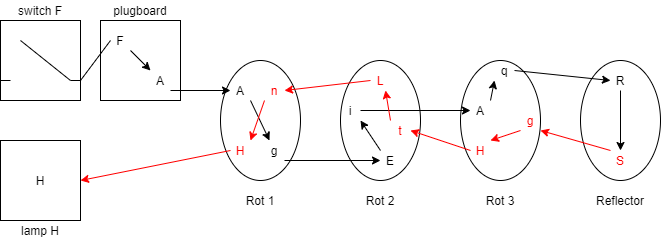
\includegraphics[width = 350pt]{Enigma.png}
\end{figure}

Per costruzione una lettera non è mai cifrata con se stessa. Questa proprietà e quella di riflessione sono state utilissime nel rompere questo sistema.

I rotori non sono fissi, per ogni lettera battuta il primo fa uno scatto, dopo 26 battute il secondo rotore fa uno scatto, dopo $26 \cdot 26$ battute fa uno scatto il terzo rotore. Ad ogni passo quindi la configurazione cambia.

Le permutazioni sono 26 per il primo rotore rispetto al secondo, 26 del secondo rispetto al terzo, 26 del terzo rispetto al riflettore: $26 \cdot 26 \cdot 26 = 17'576$ chiavi se i rotori sono immutabili e noti a chiunque ne avesse una copia. Si aumentano quindi le chiavi scambiando l'ordine dei rotori, quindi si sale a $2^6 \cdot 3! > 10^5$.

Aggiungendo le plugboard si possono scambiare 6 coppie di caratteri per ogni trasmissione, si arriva quindi ad una sequenza di 12 caratteri per descrivere il cablaggio: le combinazioni possibili sono $\binom{26}{12} \approx 10^7$. Scelte le lettere va scelta la loro ordinazione: $12!$, in realtà meno perché molte permutazioni lasciano lo stesso effetto: AB CD = CD AB, ma anche AB = BA, quindi le $6!$ disposizioni delle coppie sono uguali, si ottiene quindi $\binom{26}{12} \cdot \frac{12!}{6! \cdot 2^6} > 10^11$ (10 milioni di miliardi)

Un conteggio alternativo sarebbe: si scelgono 6 coppie di variabili in :
$$ \binom{26}{2} \binom{24}{2} \binom{22}{2} \binom{20}{2} \binom{18}{2} \binom{16}{2} = \frac{26!}{2^6 \cdot 6!} = \binom{26}{12} \cdot \frac{12!}{2^6} $$
dividiamo per le $6!$ permutazioni delle coppie:
$$ \binom{26}{12} \cdot \frac{12!}{2^6 \cdot 6!} $$

La macchina Enigma usata durante la $2^{a}$ guerra mondiale forniva invece 8 rotori in dotazione tra i quali sceglierne 3 e le coppie da scambiare nella plugboard divennero 10.

Ogni reparto disponeva di un libro con l'elenco delle chiavi: assetto dei rotori, quali rotori, in quale ordine e quali coppie connettere con la plugboard. Con l'assetto iniziale si trasmetteva la nuova chiave del messaggio indicante l'assetto per quella trasmissione. La difficoltà stava nella velocità necessaria in quanto il sistema cambiava continuamente. Portò alla creazione di COLOSSUS (1944) che fu un prototipo embrionale dei successivi calcolatori elettronici.